
\documentclass[../../../all/physics-standard_questions_all.tex]{subfiles}

\graphicspath{{../../../../figures/}}

\begin{document}

図1のように，真空中に，極板面積$S$，極板間隔$d$の平行平板コンデンサがあり，
電荷$Q$を与えてある．真空の誘電率を$\varepsilon_0$とし，端の効果は無視する．

\begin{enumerate}

    \item 電位差（電圧）$V_1$，および容量$C_1$を求めよ．

    \item 図\ref{q_circuit-extent_06_01}のコンデンサの極板間を
        比誘電率$\varepsilon_r$の誘電体で満たす（図\ref{q_circuit-extent_06_02}）．このときの電位差
        （電圧）$V_2$，および容量$C_2$を求めよ．

    \item 図\ref{q_circuit-extent_06_01}のコンデンサの極板間のちょうど下半分の領域を
        比誘電率$\varepsilon_r$の誘電体で満たす（図\ref{q_circuit-extent_06_03}）．このときの電位差
        （電圧）$V_3$，および容量$C_3$を求めよ．

    \item 図\ref{q_circuit-extent_06_01}のコンデンサの極板間のちょうど右半分の領域を
        比誘電率$\varepsilon_r$の誘電体で満たす（図\ref{q_circuit-extent_06_04}）．このときの電位差
        （電圧）$V_4$，および容量$C_4$を求めよ．

\end{enumerate}

\setcounter{figure}{0}

\vspace{0.8\baselineskip}
{\centering
    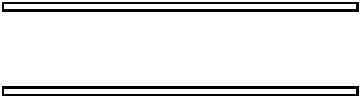
\includegraphics{q_circuit-extent_06_01/physics-standard_questions_circuit-extent_06_01_tikz.pdf}
    \captionof{figure}{} \label{q_circuit-extent_06_01}
\par}

\vspace{\baselineskip}

{\centering
    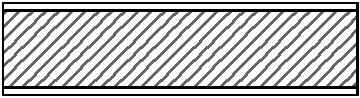
\includegraphics{q_circuit-extent_06_02/physics-standard_questions_circuit-extent_06_02_tikz.pdf}
    \captionof{figure}{} \label{q_circuit-extent_06_02}
\par}

\vspace{\baselineskip}

{\centering
    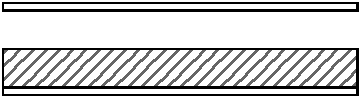
\includegraphics{q_circuit-extent_06_03/physics-standard_questions_circuit-extent_06_03_tikz.pdf}
    \captionof{figure}{} \label{q_circuit-extent_06_03}
\par}

\vspace{\baselineskip}

{\centering
    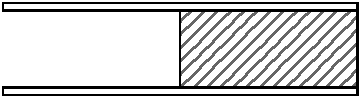
\includegraphics{q_circuit-extent_06_04/physics-standard_questions_circuit-extent_06_04_tikz.pdf}
    \captionof{figure}{} \label{q_circuit-extent_06_04}
\par}

\vspace{\baselineskip}

\end{document}
